\documentclass[../main]{subfiles}
\begin{document}

\graphicspath{{../figures/}}

\section{提案手法}
\subsection{対象とするシステムの概要}
次のようにすべての図表は必ず本文中で引用して説明する.
\reffig{logo}はロゴである.
提案手法のコンセプトは以下のとおりである.
点検員は点検時に聞こえる音を過去のその地点での正常音と比較することで,異常の検出を行っている.
本研究では,地点ごとの正常音をマッピングするニューラルネットワークを正常音を用いて学習し,点検時は,
聞こえた音とマッピングされた正常音を比較することで異常の検出を行う.



\begin{equation}
  r = \left\{
    \begin{array}{cc}
      10   & \text{if success} \\
      - 10 & \text{if fail}    \\
      - d  & \text{else}
    \end{array}
  \right. \text{.}
\end{equation}

\begin{figure}[tb]
  \centering
  
\includegraphics[keepaspectratio, width=0.8\linewidth]{utlogo.pdf}
  \caption{ロゴ}
  \labfig{logo}
\end{figure}

\subsection{ニューラルネットワークによる正常音のマッピング}
ニューラルネットワークとは,人間の脳の神経細胞を模倣した計算モデルであり,入力層,中間層,出力層から構成され,
各層のノード間の結合には重みが設定されている.
これらの重みを学習することで,入力データから出力データを予測することができる.
本研究では,入力層にはロボットの自己位置座標を,出力層にはその地点での正常音の特徴量を与え,学習時には,異常音源を含まない経路でロボットを走行させ,
運用時には,学習したモデルを用いて検査対象となる経路を走行させる.
\subsection{SAM optimizer}
SAM optimizerは,Sharpness-Aware Minimizationの略であり,モデルの汎化性能を向上させるための最適化手法である.
SAM optimizerは,モデルの重みの更新時に,重みの変化に対する損失関数の変化が小さくなるように重みの更新を行うことで,
汎化性能を向上させることを目的とした最適化手法である.
本研究では,音のマッピングを行うことをコンセプトとして挙げており,座標の変化に対して出力である音の変化が滑らかになるように,
モデルの学習を行うために,SAM optimizerを用いる.
\subsection{短時間フーリエ変換}
本研究では,座標ごとに聞こえる音をマッピングすることをコンセプトとしているが,音圧のデータは時間ずれの影響を非常に受けやすいことから,音圧の時系列データから
定常的な特徴量を抽出する必要がある.
そのため,本研究では,音圧の時系列データから短時間フーリエ変換を行い,更にメルフィルタバンクの処理を適用したメルスペクトログラムを特徴量として用いる.
\subsection{異常音座標の推定}

\begin{figure}[t]
  \centering
  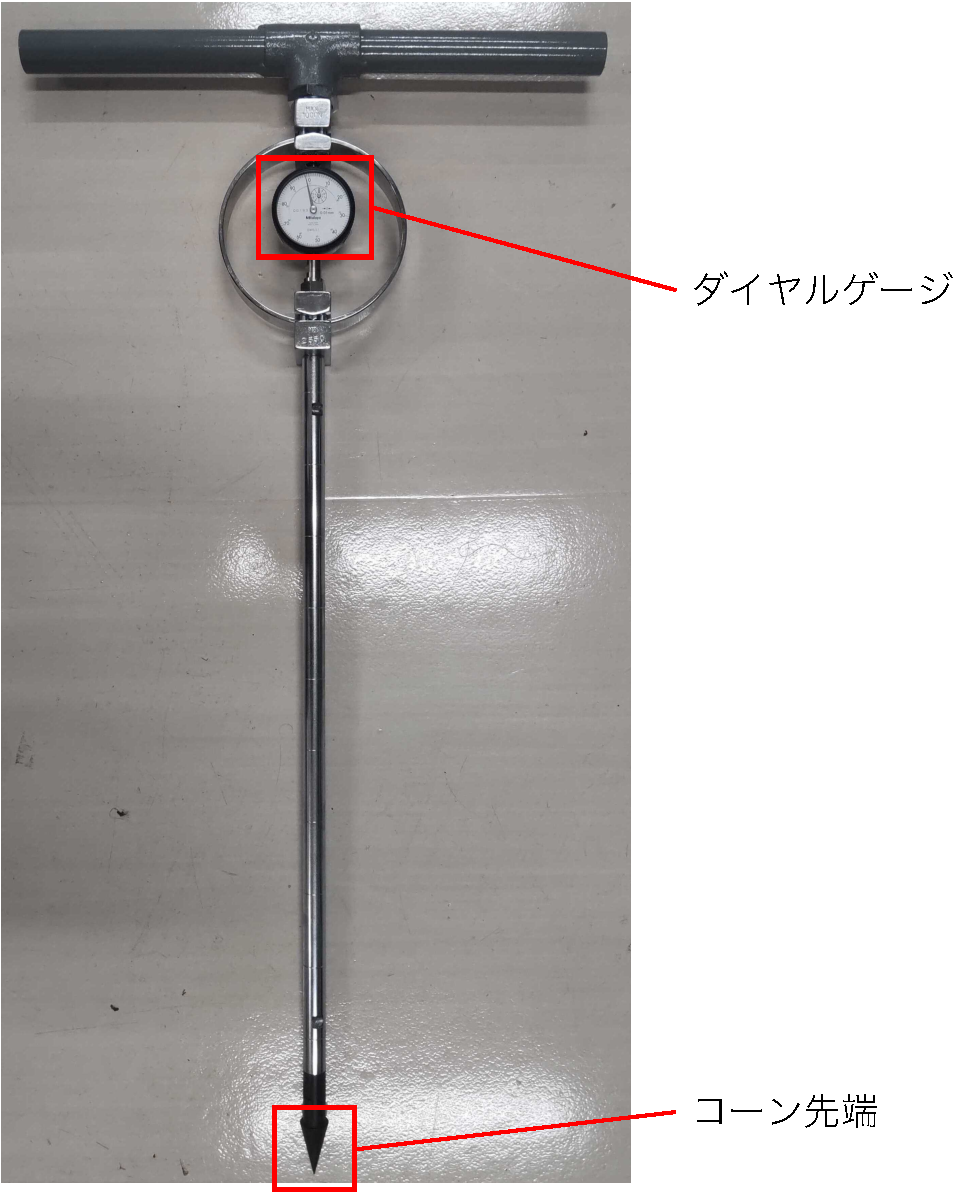
\includegraphics[keepaspectratio, width=0.5\linewidth]{cone_penetrometer.pdf}
  \caption{コーンペネトロメータ}
  \labfig{cone_penetrometer}
\end{figure}

\end{document}
